
\documentclass[letterpaper,hide notes,xcolor={table,svgnames},pdftex]{beamer}
\def\showexamples{t}


%\usepackage[svgnames]{xcolor}

%% Demo talk
%\documentclass[letterpaper,notes=show]{beamer}

\usecolortheme{crane}
\setbeamertemplate{navigation symbols}{}

\usetheme{MyPittsburgh}
%\usetheme{Frankfurt}

%\usepackage{tipa}

\usepackage{hyperref}
\usepackage{graphicx,xspace}
\usepackage[normalem]{ulem}

\newcommand\SF[1]{$\bigstar$\footnote{SF: #1}}



\newcounter{tmpnumSlide}
\newcounter{tmpnumNote}

% old question code
%\newcommand\question[1]{{$\bigstar$ \small \onlySlide{2}{#1}}}
% \newcommand\nquestion[1]{\ifdefined \presentationonly \textcircled{?} \fi \note{\par{\Large \textbf{?}} #1}}
% \newcommand\nanswer[1]{\note{\par{\Large \textbf{A}} #1}}


 \newcommand\mnote[1]{%
   \addtocounter{tmpnumSlide}{1}
   \ifdefined\showcues {~\tiny\fbox{\arabic{tmpnumSlide}}}\fi
   \note{\setlength{\parskip}{1ex}\addtocounter{tmpnumNote}{1}\textbf{\Large \arabic{tmpnumNote}:} {#1\par}}}

\newcommand\mmnote[1]{\note{\setlength{\parskip}{1ex}#1\par}}

%\newcommand\mnote[2][]{\ifdefined\handoutwithnotes {~\tiny\fbox{#1}}\fi
% \note{\setlength{\parskip}{1ex}\textbf{\Large #1:} #2\par}}

%\newcommand\mnote[2][]{{\tiny\fbox{#1}} \note{\setlength{\parskip}{1ex}\textbf{\Large #1:} #2\par}}

\newcommand\mquestion[2]{{~\color{red}\fbox{?}}\note{\setlength{\parskip}{1ex}\par{\Large \textbf{?}} #1} \note{\setlength{\parskip}{1ex}\par{\Large \textbf{A}} #2\par}\ifdefined \presentationonly \pause \fi}

\newcommand\blackboard[1]{%
\ifdefined   \showblackboard
  {#1}
  \else {\begin{center} \fbox{\colorbox{blue!30}{%
         \begin{minipage}{.95\linewidth}%
           \hspace{\stretch{1}} Some space intentionally left blank; done at the blackboard.%
         \end{minipage}}}\end{center}}%
         \fi%
}



%\newcommand\q{\tikz \node[thick,color=black,shape=circle]{?};}
%\newcommand\q{\ifdefined \presentationonly \textcircled{?} \fi}

\usepackage{listings}
\lstset{%
  keywordstyle=\bfseries,
  aboveskip=15pt,
  belowskip=15pt,
  captionpos=b,
  identifierstyle=\ttfamily,
  escapeinside={(*@}{@*)},
  stringstyle=\ttfamiliy,
  frame=lines,
  numbers=left, basicstyle=\scriptsize, numberstyle=\tiny, stepnumber=0, numbersep=2pt}

\usepackage{siunitx}
\newcommand\sius[1]{\num[group-separator = {,}]{#1}\si{\micro\second}}
\newcommand\sims[1]{\num[group-separator = {,}]{#1}\si{\milli\second}}
\newcommand\sins[1]{\num[group-separator = {,}]{#1}\si{\nano\second}}
\sisetup{group-separator = {,}, group-digits = true}

%% -------------------- tikz --------------------
\usepackage{tikz}
\usetikzlibrary{positioning}
\usetikzlibrary{arrows,backgrounds,automata,decorations.shapes,decorations.pathmorphing,decorations.markings,decorations.text}

\tikzstyle{place}=[circle,draw=blue!50,fill=blue!20,thick, inner sep=0pt,minimum size=6mm]
\tikzstyle{transition}=[rectangle,draw=black!50,fill=black!20,thick, inner sep=0pt,minimum size=4mm]

\tikzstyle{block}=[rectangle,draw=black, thick, inner sep=5pt]
\tikzstyle{bullet}=[circle,draw=black, fill=black, thin, inner sep=2pt]

\tikzstyle{pre}=[<-,shorten <=1pt,>=stealth',semithick]
\tikzstyle{post}=[->,shorten >=1pt,>=stealth',semithick]
\tikzstyle{bi}=[<->,shorten >=1pt,shorten <=1pt, >=stealth',semithick]

\tikzstyle{mut}=[-,>=stealth',semithick]

\tikzstyle{treereset}=[dashed,->, shorten >=1pt,>=stealth',thin]

\usepackage{ifmtarg}
\usepackage{xifthen}
\makeatletter
% new counter to now which frame it is within the sequence
\newcounter{multiframecounter}
% initialize buffer for previously used frame title
\gdef\lastframetitle{\textit{undefined}}
% new environment for a multi-frame
\newenvironment{multiframe}[1][]{%
\ifthenelse{\isempty{#1}}{%
% if no frame title was set via optional parameter,
% only increase sequence counter by 1
\addtocounter{multiframecounter}{1}%
}{%
% new frame title has been provided, thus
% reset sequence counter to 1 and buffer frame title for later use
\setcounter{multiframecounter}{1}%
\gdef\lastframetitle{#1}%
}%
% start conventional frame environment and
% automatically set frame title followed by sequence counter
\begin{frame}%
\frametitle{\lastframetitle~{\normalfont(\arabic{multiframecounter})}}%
}{%
\end{frame}%
}
\makeatother

\makeatletter
\newdimen\tu@tmpa%
\newdimen\ydiffl%
\newdimen\xdiffl%
\newcommand\ydiff[2]{%
    \coordinate (tmpnamea) at (#1);%
    \coordinate (tmpnameb) at (#2);%
    \pgfextracty{\tu@tmpa}{\pgfpointanchor{tmpnamea}{center}}%
    \pgfextracty{\ydiffl}{\pgfpointanchor{tmpnameb}{center}}%
    \advance\ydiffl by -\tu@tmpa%
}
\newcommand\xdiff[2]{%
    \coordinate (tmpnamea) at (#1);%
    \coordinate (tmpnameb) at (#2);%
    \pgfextractx{\tu@tmpa}{\pgfpointanchor{tmpnamea}{center}}%
    \pgfextractx{\xdiffl}{\pgfpointanchor{tmpnameb}{center}}%
    \advance\xdiffl by -\tu@tmpa%
}
\makeatother
\newcommand{\copyrightbox}[3][r]{%
\begin{tikzpicture}%
\node[inner sep=0pt,minimum size=2em](ciimage){#2};
\usefont{OT1}{phv}{n}{n}\fontsize{4}{4}\selectfont
\ydiff{ciimage.south}{ciimage.north}
\xdiff{ciimage.west}{ciimage.east}
\ifthenelse{\equal{#1}{r}}{%
\node[inner sep=0pt,right=1ex of ciimage.south east,anchor=north west,rotate=90]%
{\raggedleft\color{black!50}\parbox{\the\ydiffl}{\raggedright{}#3}};%
}{%
\ifthenelse{\equal{#1}{l}}{%
\node[inner sep=0pt,right=1ex of ciimage.south west,anchor=south west,rotate=90]%
{\raggedleft\color{black!50}\parbox{\the\ydiffl}{\raggedright{}#3}};%
}{%
\node[inner sep=0pt,below=1ex of ciimage.south west,anchor=north west]%
{\raggedleft\color{black!50}\parbox{\the\xdiffl}{\raggedright{}#3}};%
}
}
\end{tikzpicture}
}


%% --------------------

%\usepackage[excludeor]{everyhook}
%\PushPreHook{par}{\setbox0=\lastbox\llap{MUH}}\box0}

%\vspace*{\stretch{1}

%\setbox0=\lastbox \llap{\textbullet\enskip}\box0}

\setlength{\parskip}{\fill}

\newcommand\noskips{\setlength{\parskip}{1ex}}
\newcommand\doskips{\setlength{\parskip}{\fill}}

\newcommand\xx{\par\vspace*{\stretch{1}}\par}
\newcommand\xxs{\par\vspace*{2ex}\par}
\newcommand\tuple[1]{\langle #1 \rangle}
\newcommand\code[1]{{\sf \footnotesize #1}}
\newcommand\ex[1]{\uline{Example:} \ifdefined \presentationonly \pause \fi
  \ifdefined\showexamples#1\xspace\else{\uline{\hspace*{2cm}}}\fi}

\newcommand\ceil[1]{\lceil #1 \rceil}


\AtBeginSection[]
{
   \begin{frame}
       \frametitle{Outline}
       \tableofcontents[currentsection]
   \end{frame}
}



\pgfdeclarelayer{edgelayer}
\pgfdeclarelayer{nodelayer}
\pgfsetlayers{edgelayer,nodelayer,main}

\tikzstyle{none}=[inner sep=0pt]
\tikzstyle{rn}=[circle,fill=Red,draw=Black,line width=0.8 pt]
\tikzstyle{gn}=[circle,fill=Lime,draw=Black,line width=0.8 pt]
\tikzstyle{yn}=[circle,fill=Yellow,draw=Black,line width=0.8 pt]
\tikzstyle{empty}=[circle,fill=White,draw=Black]
\tikzstyle{bw} = [rectangle, draw, fill=blue!20, 
    text width=4em, text centered, rounded corners, minimum height=2em]
    
    \newcommand{\CcNote}[1]{% longname
	This work is licensed under the \textit{Creative Commons #1 3.0 License}.%
}
\newcommand{\CcImageBy}[1]{%
	\includegraphics[scale=#1]{creative_commons/cc_by_30.pdf}%
}
\newcommand{\CcImageSa}[1]{%
	\includegraphics[scale=#1]{creative_commons/cc_sa_30.pdf}%
}
\newcommand{\CcImageNc}[1]{%
	\includegraphics[scale=#1]{creative_commons/cc_nc_30.pdf}%
}
\newcommand{\CcGroupBySa}[2]{% zoom, gap
	\CcImageBy{#1}\hspace*{#2}\CcImageNc{#1}\hspace*{#2}\CcImageSa{#1}%
}
\newcommand{\CcLongnameByNcSa}{Attribution-NonCommercial-ShareAlike}

\newenvironment{changemargin}[1]{% 
  \begin{list}{}{% 
    \setlength{\topsep}{0pt}% 
    \setlength{\leftmargin}{#1}% 
    \setlength{\rightmargin}{1em}
    \setlength{\listparindent}{\parindent}% 
    \setlength{\itemindent}{\parindent}% 
    \setlength{\parsep}{\parskip}% 
  }% 
  \item[]}{\end{list}} 



\usepackage{alltt}

\title{Lecture 22 --- Debugging III }

\author{Jeff Zarnett \\ \small \texttt{jzarnett@uwaterloo.ca}}
\institute{Department of Electrical and Computer Engineering \\[-1ex]
  University of Waterloo}
\date{\today}

\begin{document}

\begin{frame}
  \titlepage

  \vfill
  \begin{center}
    \CcGroupBySa{0.83}{0.95ex}\\
                  {\tiny\CcNote{\CcLongnameByNcSa}}
                  \vspace*{-2.5ex}
  \end{center}

\end{frame}

\begin{frame}
\frametitle{Debugging Parallel Programming}
\begin{changemargin}{1cm}
Bugs are our enemies.

Last time we talked about Heisenbugs and race conditions.

Race condition: the order of the computation steps matters and it's possible that if the steps execute in a certain order, the result is incorrect.

\end{changemargin}
\end{frame}


\begin{frame}
\frametitle{Debugging Parallel Programming}
\begin{changemargin}{1cm}

Let's imagine we have an instance of an object \texttt{Location} that has two co-ordinates, \texttt{x} and \texttt{y}. 


\texttt{location.setX(5);\quad\quad location.setX(10);}
\texttt{location.setY(7);\quad\quad location.setY(0);}

\end{changemargin}
\end{frame}

\begin{frame}
\frametitle{Location Example}
\begin{changemargin}{1cm}
Even if each method is atomic, we cannot guarantee an order.

Consider this order:
\begin{enumerate}
	\item Set \texttt{x} to 5
	\item Set \texttt{x} to 10
	\item Set \texttt{y} to 0
	\item Set \texttt{y} to 7
\end{enumerate} 

Result: $(10, 7)$ - Inconsistent! \mnote{Now our data is inconsistent! There was never a location of  in our data set - it should be either $(5, 7)$ or $(10, 0)$, but not half of one and half of another.}

\end{changemargin}
\end{frame}


\begin{frame}
\frametitle{Location Example}
\begin{changemargin}{1cm}
This only occurs some of the time - Heisenbug!

Most of the time, the answer is right.

Debugging or printing statements might hide the error.

\mnote{Furthermore, when trying to debug it, for example, adding print statements that output to the console things like ``setting x to 10'' will change the execution order and the speed of execution of the system. It's possible that adding that debug information to thread 2 will slow it down enough that it always executes after thread 1, preventing the problem from occurring while you debug. How frustrating!}

\end{changemargin}
\end{frame}

\begin{frame}
\frametitle{Location Example}
\begin{changemargin}{1cm}
Is our example realistic?

Imagine two users editing contact information for a vendor.

Multithreaded bug - are single threaded programs immune?

\end{changemargin}
\end{frame}

\begin{frame}
\frametitle{Parallel Bugs in Single Threaded Systems}
\begin{changemargin}{1cm}
Let's use an example from the labs: step counter.

Even a simple operation like \texttt{steps++;} is broken down into smaller operations.

You've just detected a step. Let's assume the current value of the variable is 4.

\end{changemargin}
\end{frame}

\begin{frame}
\frametitle{Parallel Bugs in Single Threaded Systems}
\begin{changemargin}{1cm}
Normally, \texttt{steps++;} works like this:

\begin{enumerate}
	\item Read the current value of \texttt{steps} (read 4)
	\item Add 1 to the value (now it's 5)
	\item Write the changed value back to memory (write 5)
\end{enumerate}

\end{changemargin}
\end{frame}


\begin{frame}
\frametitle{Parallel Bugs in Single Threaded Systems}
\begin{changemargin}{1cm}
Imagine an interrupt comes at the worst possible time.

The user presses the reset button. Should set \texttt{steps} = 0.

\begin{enumerate}
	\item Read the current value of \texttt{steps} (read 4)
	\item Add 1 to the value (now it's 5)
	\item INTERRUPT (control goes to the interrupt handler)
	\item Write 0 to the total number of steps (write 0)
	\item END INTERRUPT (control returns to where it was)
	\item Write the changed value back to memory (write 5)
\end{enumerate}

\end{changemargin}
\end{frame}

\begin{frame}
\frametitle{Parallel Bugs in Single Threaded Systems}
\begin{changemargin}{1cm}

If the interrupt came after ``write 5'', \texttt{steps} would be 0. OK.

If the interrupt came before ``read 4'', \texttt{steps} would be 1. OK.

At the end of the last slide's sequence, \texttt{steps} is 5. Wrong! \mnote{At the end of this execution sequence, the variable \texttt{steps} shows 5, but it should show 0 (or 1), but instead it shows 5, which is certainly wrong. The user pressed the reset button but the step count did not reset! If the reset interrupt had occurred before reading the variable, the step count would have been reset, and then a step detected and the count goes up to 1. If the interrupt had occurred after writing the value 5 to the variable we would see the step count set to 0 as is expected. If it occurred after the read but before the write, there is an error and the changes the interrupt handler made were lost.}

Wait a minute -- changes overwritten? This looks familiar...

\end{changemargin}
\end{frame}

\begin{frame}
\frametitle{Parallel Bugs in Single Threaded Systems}
\begin{changemargin}{1cm}

\begin{center}
	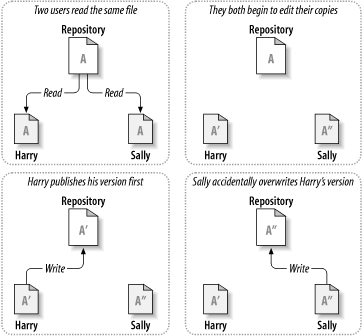
\includegraphics[width=.5\textwidth]{images/ch02dia2.png}
	\hfill {\tiny \url{http://svnbook.red-bean.com/en/1.6/svn.basic.version-control-basics.html}}
\end{center} \mnote{Yes, it's very much the same problem as when Harry was overwritten by Sally. And what did we do in this situation (as our first attempt)? We used the lock-modify-unlock model. And that's exactly what happens in a lot of software. Back to our earlier example:}

\end{changemargin}
\end{frame}

\begin{frame}
\frametitle{Solution: Lock-Modify-Unlock}
\begin{changemargin}{1cm}

Back to our earlier example:

\begin{columns}

	\column{0.35\textwidth}

		\texttt{lock(location);} 
		\texttt{location.setX(5);}
		\texttt{location.setY(7);}
		\texttt{unlock(location);}
		
	\column{0.35\textwidth}

		\texttt{lock(location);} 
		\texttt{location.setX(10);}
		\texttt{location.setY(0);}
		\texttt{unlock(location);}

\end{columns}

\end{changemargin}
\end{frame}


\begin{frame}
\frametitle{Solution: Lock-Modify-Unlock}
\begin{changemargin}{1cm}

How the \texttt{lock} and \texttt{unlock} functions work is beyond the scope of this course; we are just interested in the concept.

Thread 1 locks the \texttt{location} object. Thread 2's attempt to lock the same object cannot succeed until Thread 1 unlocks it.

Thread 2 must wait.

\end{changemargin}
\end{frame}

\begin{frame}
\frametitle{Solution: Lock-Modify-Unlock}
\begin{changemargin}{1cm}

At the end of execution, the data could be $(5,7)$ or $(10,0)$.

It cannot be some mixup of the two like $(10, 7)$. 
\mnote{Relating all of this back to debugging: if you find some record or object that is in an inconsistent state (or some other kind of Heisenbug or shared data), then probably the error can be resolved with locking and unlocking the object.}

\end{changemargin}
\end{frame}

\begin{frame}
\frametitle{Debugging Embedded Systems}
\begin{changemargin}{1cm}

Embedded systems present a number of special debugging challenges.

There may be no console to print debug messages (or maybe no screen).


\end{changemargin}
\end{frame}

\begin{frame}
\frametitle{Embedded Systems diagram}

\begin{center}
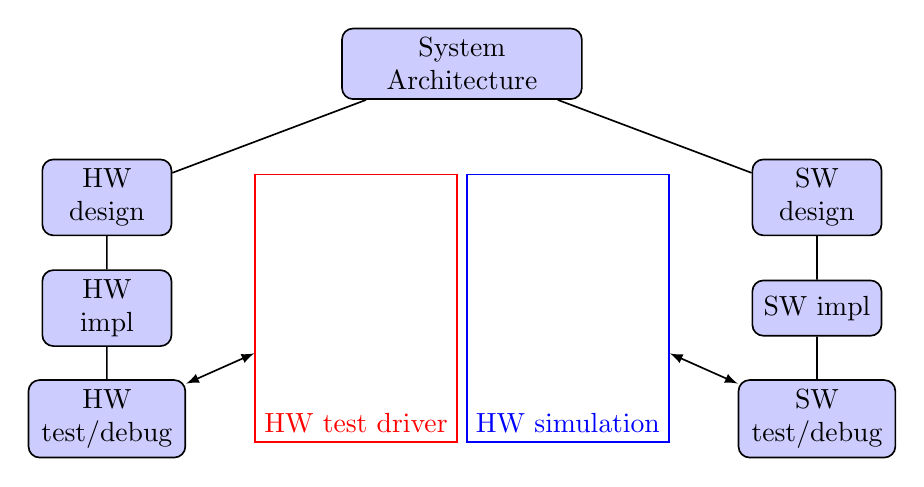
\begin{tikzpicture}[auto,node distance=4em,
                    semithick,initial text=]
  \node [bw,text width=8em] (arch) {System\\Architecture}; 

  \node [red,below left of=arch, xshift=-1em, draw, yshift=-6em, text height=9em] (hwtd) {HW test driver};
  \node [blue,below right of=arch, xshift=1em, draw, yshift=-6em, text height=9em] (swtd) {HW simulation};

  \node [bw, left of=hwtd,xshift=-5em,yshift=4em] (hwd) {HW design};
  \node [bw, below of=hwd] (hwi) {HW impl};
  \node [bw, below of=hwi,text width=5em] (hwt) {HW test/debug};

  \node [bw, right of=swtd,xshift=5em,yshift=4em] (swd) {SW design};
  \node [bw, below of=swd] (swi) {SW impl};
  \node [bw, below of=swi,text width=5em] (swt) {SW test/debug};

  \path[draw] (arch) -- (hwd)
        (arch) -- (swd)
        (hwd) -- (hwi)
        (swd) -- (swi)
        (hwi) -- (hwt)
        (swi) -- (swt);

   \path[draw,<->,>=latex] (hwt) -- (hwtd);
   \path[draw,<->,>=latex] (swt) -- (swtd);
\end{tikzpicture}
\end{center}

\end{frame}


\begin{frame}
\frametitle{Debugging Embedded Systems: Simulation}
\begin{changemargin}{1cm}

Simulate!

Reproduce the problem in the emulator (if possible).

Simulators often have consoles, and we can use a debugger.

Not always available.


\end{changemargin}
\end{frame}

\begin{frame}
\frametitle{Debugging Embedded Systems: Actuators}
\begin{changemargin}{1cm}

Use your actuators.

Make LEDs flash, or make noise.

Show an error code on a numeric display. (Microwave?)

Famous example: BIOS Power On Self Test (POST) in PCs. \mnote{The POST would execute and then beep to indicate what, if anything, was wrong with the system. One beep meant all tests passed; different sequences of beeps indicated other issues: memory error, no boot device found, keyboard absent, etc. Once you identify what error code the system reported, you are closer to solving the problem.}

\end{changemargin}
\end{frame}

\begin{frame}
\frametitle{Debugging Embedded Systems: Debugging Functions}
\begin{changemargin}{1cm}

Add debugging functions.

Allows you to put the system in a specific state.

Circumvent normal rules of the system.

You can use a physical button or software input to do it. \mnote{You might use a physical button (or sequence of button presses) to load some specific data into memory (or a function) to use in debugging. In other cases, you execute some software command(s) to trigger the debug function. }

Real life example: cheat codes (\texttt{iddqd}). \mnote{This was the ``god mode'' cheat code in the original DOOM game.}

\end{changemargin}
\end{frame}

\begin{frame}
\frametitle{Debugging Embedded Systems: Standard Interface}
\begin{changemargin}{1cm}

Use a standard interface.

JTAG is a standard interface for testing and I/O in many embedded systems. \mnote{Joint Test Action Group}

It's possible (but not necessarily a good idea), to use the JTAG interface to flash your XBOX 360.

In ECE~327, you'll learn more about how JTAG works. In this course, you don't need to know any details about JTAG.

\end{changemargin}
\end{frame}





\end{document}
